\chapter{Signature Method}   
\label{ch:signature-method}

This chapter delves into the intricacies of the signature method, a robust tool for analyzing paths and curves. We explore its fundamental concepts, including tensor algebra and the definition of the signature along with its properties. Additionally, we investigate the logarithmic signature for path representation. The chapter culminates with numerical examples illustrating the method's application in shape analysis.

\section{Fundamentals of the Signature Method}
\label{sec:signature-fundamentals}

This section delves into the foundational aspects of the signature method, including tensor algebra, the definition of the signature, and its properties.

\subsection{Tensor Algebra and Its Dual Space}
\label{subsec:tensor-algebra}

Within the context of a finite-dimensional vector space \(V\) with dimension \(d\), the tensor algebra \(T(V)\) encompasses all tensor powers of \(V\):
\begin{equation}
    T(V) := \bigoplus_{n=0}^{\infty} V^{\otimes n} = \mathbb{R} \oplus V \oplus (V \otimes V) \oplus (V \otimes V \otimes V) \oplus \cdots,
\end{equation}
where \(V^{\otimes n}\) denotes the \(n\)-th tensor product of \(V\) and \(V^{\otimes 0} = \mathbb{R}\) \cite{chenAlgebrasIteratedPath1971}.

The dual space of the tensor algebra, denoted \(T((V)) := T(V)^*\) or \(T(V^*)\), represents the domain of formal power series in \(d\) non-commuting variables, represented by the set \(\{e_1, \ldots, e_d\}\) \cite{chenIntegrationPathsGeometric1957}.

In a \(d\)-dimensional vector space, tensor series are depicted as infinite vectors indexed by words from the alphabet \(\{1, \ldots, d\}\). Each word \(w = i_1 \cdots i_n\), with \(i_j\) drawn from \(\{1, \ldots, d\}\), corresponds to a fundamental element \(e_w = e_{i_1} \otimes \cdots \otimes e_{i_n}\) \cite{chevyrevPrimerSignatureMethod2016}. This conceptual framework serves as the cornerstone for defining iterated integrals of a path in \(\mathbb{R}^d\).

\subsection{Definition of the Signature}
\label{subsec:signature-definition}

For a smooth path \(x : [s, t] \to \mathbb{R}^d\) over \( [s, t] \subset [0, 1]\), the \(n\)-fold iterated integral for a word \(w = i_1 \cdots i_n\) is defined as:
\begin{equation}
\langle S(x)_{s,t}, e_w \rangle = \int_{s < u_n < \cdots < u_1 < t} dx_{u_1}^{i_1} \cdots dx_{u_n}^{i_n}.
\end{equation}
This provides geometric insights into the path \(x\) \cite{lyonsRoughPathsSignatures2014}.

The signature \(S(x)_{s,t}\) of \(x\) over \( [s, t] \) is represented by the tensor series:
\begin{equation}
S(x)_{s,t} = 1 + \sum_{|w| \geq 1} \langle S(x)_{s,t}, e_w \rangle e_w \in T((\mathbb{R}^d)^*),
\end{equation}
aggregating its iterated integrals \cite{lyonsRadiusConvergenceLogarithmic2006}.

To enhance computational efficiency, we truncate the signature at level \( n \), capturing terms up to word length \( n \). The truncated signature \( S(x)_{s,t}^{(n)} \) is given by:
\begin{equation}
S(x)_{s,t}^{(n)} = 1 + \sum_{1 \leq |w| \leq n} \langle S(x)_{s,t}, e_w \rangle e_w,
\end{equation}
where \( |w| \) represents the word length \cite{reizensteinCalculationIteratedIntegralSignatures2017}.

The number of terms in \( S(x)_{s,t}^{(n)} \) is calculated as:
\begin{equation}
M = \frac{d(d^n - 1)}{d - 1},
\label{eq:logsig-terms}
\end{equation}
where \(d\) is the path's dimension, crucial for balancing computational efficiency and information capacity \cite{reizensteinIisignatureLibraryEfficient2018}.

%%%%%%%%%%%%%%%%%%%%%%%%%%%%%%%%%%%%%%%%%%%%%%%%%%%%%%%%%%%%%%%%

\subsection{Signatures on Piecewise Linear Paths}
\label{subsec:signature-piecewise-linear}

For linear paths in \(\mathbb{R}^d\), such as \(x(t) = a \cdot t + b\), the \(n\)-fold iterated integral for a word \(w = i_1 \cdots i_n\) simplifies to:
\begin{equation}
\langle S(x)_{s,t}, e_w \rangle = \frac{(t - s)^n}{n!} \prod_{k=1}^n a_{i_k}.
\end{equation}

Following prior work \cite{reizensteinCalculationIteratedIntegralSignatures2017, celledoniSignaturesShapeAnalysis2019}, the signature for a linear path is derived as:
\begin{equation}
S(x)_{s,t} = 1 + \sum_{|w|\geq 1} \frac{(t-s)^n}{n!} \prod^n_{k=1} a_{ik}e_w = \exp_{\otimes}((t-s)a).
\label{eq:signature_linear}
\end{equation}

Applying Chen's Identity \cite{chenIteratedIntegralsExponential1954}, for a path \(x\) and \(0 \leq s \leq u \leq t \leq 1\), yields:
\begin{equation}
S(x)_{s,u} \otimes S(x)_{u,t} = S(x)_{s,t}.
\label{eq:chens-rule}
\end{equation}

For a piecewise linear path, combining equation \eqref{eq:signature_linear} with \eqref{eq:chens-rule} results in the signature:
\begin{equation}
S(x)_{s,t} = \bigotimes_{k=1}^{m} \exp_{\otimes}(\Delta t_k a_k) = \exp_{\otimes}(\Delta t_1a_1) \otimes \dots \otimes \exp_{\otimes}(\Delta t_ma_m),
\end{equation}
where \(\Delta t_k = t_k - t_{k-1}\) represents the lengths of the time intervals, and \(a_1, \ldots, a_m\) are the slopes of the segments.

%%%%%%%%%%%%%%%%%%%%%%%%%%%%%%%%%%%%%%%%%%%%%%%%%%%%%%%%%%%%%%%%

\subsection{Signature for a Smooth Curve in a Lie Group}
\label{subsec:signature-lie-group}

Following \cite{celledoniSignaturesShapeAnalysis2019, leePathSignaturesLie2020}, for a smooth curve \( c: [0, 1] \to G \) in a Lie group \( G \), the \( n \)-fold iterated integral of the signature is defined recursively, with the base \(\langle S(c)_{s,t}, 1 \rangle := 1\) and the recursive step:

\begin{equation}
\langle S(c)_{s,t}, e_{i_1},\ldots,e_{i_n} \rangle := \int_{s}^{t} \langle S(c)_{s,u}, e_{i_1},\ldots,e_{i_{n-1}} \rangle \omega^{i_n}_{c(u)}( \dot{c}(u)) du,
\end{equation}
where \( \omega^{j}_{c}(v) \) denotes the \( j \)-th component of \( \omega_{c}(v) \in \mathfrak{g} \).

For a smooth curve \( \kappa: [s_k, s_{k+1}] \to G \), where \( G = SO(3) \) or \( SE(3) \), representing the geodesic interpolation between configurations \( c_k \) and \( c_{k+1} \), the term \( \tilde{\eta}_k \) is defined as:

\begin{equation}
\tilde{\eta}_k = \frac{\log(c_{k+1}c_k^{-1})}{s_{k+1} - s_k},
\end{equation}
and the right logarithmic derivative \( \omega_\kappa (\dot \kappa)(t) = \hat{\eta}_k \) is formulated accordingly. Utilizing \( \eta_k \in \mathfrak{g} \), derived from the inverse hat map, the \( n \)-fold integrals for the signature of \( \kappa \) are given by:

\begin{equation}
\langle S(\kappa)_{s_k,s_{k+1}}, e_{i_1,\ldots,i_n} \rangle = \frac{(s_{k+1} - s_k)^n}{n!} \prod_{j=1}^n \eta_{k}^{i_j},
\end{equation}
for each appropriate index set. Consequently, the signature over the interval \( [s_k, s_{k+1}) \) is:

\begin{equation}
S(\kappa)_{s_k,s_{k+1}} = \exp_{\otimes}\left( (s_{k+1} - s_k) \tilde{\eta}_k \right).
\label{eq:signature_lie_group}
\end{equation}

This methodology extends to paths in Lie groups such as \( SO(3)^d \) and \( SE(3)^d \), by adapting the index set and employing Chen’s rule for concatenation.

%%%%%%%%%%%%%%%%%%%%%%%%%%%%%%%%%%%%%%%%%%%%%%%%%%%%%%%%%%%%%%%%

\subsection{Properties of Signature Space for Paths}
\label{subsec:signature-properties}

In the signature space of a path \(x : [0,1] \to \mathbb{R}^d\), the identity is \(S(x)_{s,s} = 1\), and its inverse is \(S_{s,t}^{-1}(x) = S_{s,t}(\overleftarrow{x})\), where \(\overleftarrow{x}(t) = x(1 - t)\) \cite{chevyrevPrimerSignatureMethod2016}. This inverse relationship is captured by Chen's identity:

\begin{equation}
S(x) \otimes S(\overleftarrow{x}) = 1.
\label{eq:chens-identity}
\end{equation}

Chen's rule indicates that the signature acts as a homomorphism from the path space under concatenation to the dual tensor algebra \cite{chenIntegrationPathsFaithful1958}. For paths \(x, y : [0,1] \rightarrow \mathbb{R}^d\), their concatenation \(x*y\) satisfies:

\begin{equation}
S(x*y)_{0,1} = S(x)_{0,1} \otimes S(y)_{0,1}
\end{equation}

Consequently, the identity for concatenation is:

\begin{equation}
S(x*\overleftarrow{x})_{0,1} = 1.
\end{equation}

For the concatenation of two paths \(c_1, c_2 : [0,1] \rightarrow G\), denoted \(c_1 * c_2\), where \(G\) represents a Lie group, the homomorphism property is preserved:

\begin{equation}
    S(c_1 * c_2)_{s,t} = S(c_1)_{s,t} \otimes S(c_2)_{s,t}.
\end{equation}

Parameterization invariance in concatenation allows for flexibility in choosing a midpoint within the interval \((0,1)\).

%%%%%%%%%%%%%%%%%%%%%%%%%%%%%%%%%%%%%%%%%%%%%%%%%%%%%%%%%%%%%%%%

\subsection{Uniqueness of the Path Signature}
\label{subsec:uniqueness-signature}

The path signature provides a unique characterization of a path, subject to certain constraints: translation, parameterization, and irreducibility \cite{chenIntegrationPathsFaithful1958}.

Translation invariance naturally arises from the signature's derivation. It stems from the manner in which iterated integrals are computed, where the differential \(dx_t = \frac{dx}{dt}dt\) effectively eliminates any dependence on the initial position of the path.

Under parameterization that maintains the path's orientation, the signature remains invariant. For any orientation-preserving diffeomorphism \(\varphi\) defined over the interval \([s,t]\), the path's signature adheres to \(S(x \circ \varphi)_{s,t} = S(x)_{s,t}\). Consequently, the signature transcends mere parameterization nuances.

Irreducibility denotes that a path cannot be expressed in a particular concatenated form involving path reversal. This notion is pivotal, as it underscores that the signature of the concatenated path \(x*y*\overleftarrow{y}*z\) mirrors that of the simpler path \(x*z\).

%%%%%%%%%%%%%%%%%%%%%%%%%%%%%%%%%%%%%%%%%%%%%%%%%%%%%%%%%%%%%%%%

\section{The Logarithmic Signature}
\label{sec:logarithmic-signature}

In the realm of signature spaces, the emergence of a group structure naturally prompts inquiries into the existence of an associated Lie algebra and a corresponding logarithmic mapping. Chen first elucidated this aspect, confirming the presence of a Lie algebra structure within signature spaces and demonstrating that the logarithmic map yields a closed subspace within the tensor algebra \cite{chenIntegrationPathsGeometric1957}. Expanding upon Chen's concept, Lyons and Sidorova described this space as a 'formal Lie algebra', providing deeper insights into the structural dynamics within the group-like environment of signature spaces \cite{lyonsRadiusConvergenceLogarithmic2006}. Building upon this foundation, we now extend our exploration from the conventional signature to the logarithmic signature. In this section, we will examine its properties and make a case for its utility in practical applications.

\subsection{The Logarithmic Signature of a Path}
\label{subsec:log-signature-path}

The logarithmic signature constitutes a powerful transformation of the path signature, offering profound insights into the geometric and analytic properties of paths. This section introduces and explores the intricacies of this transformation within the framework of formal power series.

Beginning with the foundational principles outlined in \cite{chevyrevPrimerSignatureMethod2016}, we establish the logarithmic signature as a formal power series. Represented by \(x\), the series takes the form:

\begin{equation}
x = \sum_{k=0}^\infty \sum_{i_1,\ldots,i_k \in \{1,\ldots,d\}} \lambda_{i_1,\ldots,i_k} e_{i_1} \cdots e_{i_k},
\end{equation}
where \(\lambda_0 > 0\) ensures its convergence. The logarithm of \(x\) is then defined as:

\begin{equation}
\log x = \log(\lambda_0) + \sum_{n=1}^\infty \frac{(-1)^{n}}{n} \left( \frac{x}{\lambda_0} - 1 \right)^{\otimes n},
\end{equation}
with \(\otimes n\) denoting the n-th tensor power using the tensor product \(\otimes\).

Exploring further, we illustrate the practical implications of this transformation through a concrete scenario. Consider a series \(x\) defined as:

\begin{equation}
x = 1 + \sum_{k=1}^\infty \frac{\lambda^k}{k!} e_1^{\otimes k}.
\end{equation}

A straightforward computation reveals that \(\log x = \lambda e_1\), showcasing how the logarithmic signature captures essential information from the original series while preserving finite coefficients.

The logarithmic signature of a path \(X : [s, t] \to \mathbb{R}^d\) is formally represented as \(\mathcal{LS}(X)_{s,t} := \log S(X)_{s,t}\), as per Definition 6 in \cite{chevyrevPrimerSignatureMethod2016}. This representation facilitates a deeper understanding of the path's geometric structure and analytical properties.

Moreover, Theorem 4 in the same work establishes that for any given path, the log signature can be expressed in terms of real coefficients \(\lambda_{i_1,\ldots,i_k}\), as:

\begin{equation}
\mathcal{LS}(X)_{s,t} = \sum_{k=1}^\infty \sum_{i_1,\ldots,i_k \in \{1,\ldots,d\}} \lambda_{i_1,\ldots,i_k} [e_{i_1}, [e_{i_2}, \ldots, [e_{i_{k-1}}, e_{i_k}] \ldots]].
\end{equation}

It's essential to note that these coefficients may not be unique due to the inherent lack of linear independence among certain polynomial constructs, as exemplified by the Lie bracket.

Furthermore, the injective nature of the logarithmic signature, as established in \cite{hamblyUniquenessSignaturePath2010}, underscores its significance as a unique representation of a path. This uniqueness aligns with the properties of the path's signature, emphasizing its role as a fundamental analytical tool.

Additionally, \cite{lyonsRoughPathsSignatures2014} accentuates the logarithmic signature space's flat geometry, simplifying distance computations by allowing the use of Euclidean norms. This geometric property enhances its practical utility in various analytical and computational contexts.

%%%%%%%%%%%%%%%%%%%%%%%%%%%%%%%%%%%%%%%%%%%%%%%%%%%%%%%%%%%%%%%%

\subsection{Redundancy in Standard Signature Analysis}
\label{subsec:redundancy-signature}

The issue of redundancy in standard signatures is notable. For \(n\)-fold integrals of the word \( w \), \(\langle S(x)_{s,t}, e_w \rangle\), with repetitions of letter \( i \), the signature only reflects the increment of the path \( x \)
\begin{align}
    \langle S(x)_{s,t}, e_i \rangle &= x_t - x_s, \nonumber \\
    \langle S(x)_{s,t}, e_{ii} \rangle &= \frac{(x^i_t - x^i_s)^2}{2!},  \\
    \langle S(x)_{s,t}, e_{iii} \rangle &= \frac{(x^i_t - x^i_s)^3}{3!}, \nonumber \\
    &\vdots \nonumber
\end{align}
which are just different powers of the increment. 

In the work of Ree \cite{reeLieElementsAlgebra1958}, the concept of the shuffle product is introduced to elucidate the inherent redundancy in the multiplication of signature terms. This concept is instrumental in demonstrating that the product of two such terms can be decomposed into a sum of more intricate signature terms. These terms are derived from the \((p,q)\)-shuffles of words \( i \) and \( j \), denoted as \( \text{Sh}(p,q) \). A \((p,q)\)-shuffle consists of permutations \( \sigma \) that preserve the order of the letters in both \( i \) and \( j \). Consequently, the product of the signatures of \( i \) and \( j \) can be expressed as an aggregate of all \((p,q)\)-shuffles of \( k \), represented mathematically as:

\begin{equation}
    \langle S(x)_{s,t}, e_{i_1,\ldots,i_p} \rangle \cdot \langle S(x)_{s,t}, e_{j_1,\ldots,j_q} \rangle = \sum_{\sigma \in \text{Sh}(p,q)} \langle S(x)_{s,t}, e_{k_{\sigma(1)},\ldots,k_{\sigma(p+q)}} \rangle.
\end{equation}

An exemplary case is the term for the word \( ij \), given by:

\begin{equation}
   \langle S(x)_{s,t}, e_{ij} \rangle = \langle S(x)_{s,t}, e_{ji} \rangle - \langle S(x)_{s,t}, e_i \rangle \cdot \langle S(x)_{s,t}, e_j \rangle,
\end{equation}
which does not offer additional geometric insight beyond the area encompassed by \( ji \) and the increments \( i \) and \( j \).

%%%%%%%%%%%%%%%%%%%%%%%%%%%%%%%%%%%%%%%%%%%%%%%%%%%%%%%%%%%%%%%%

\subsection{Efficiency of Logarithmic Signatures}
Logarithmic signatures, in contrast to standard signatures, eliminate redundancy and succinctly encapsulate the geometric essence of a path's signature. For a two-dimensional path, a signature \( S(x) \) truncated at level \( L = 2 \) is represented as:

\begin{equation}
S(x) = (1, S^{(1)}(x), S^{(2)}(x), S^{(1,1)}(x), S^{(2,1)}(x), S^{(1,2)}(x), S^{(2,2)}(x)).
\end{equation}

The logarithmic signature \( \mathcal{LS}(x) \), truncated at the same level, is expressed as:

\begin{equation}
\mathcal{LS}(x) = \left(S^{(1)}(x), S^{(2)}(x), \tilde{S}^{(1,2)}(x)\right),
\label{eq:logsig-truncated}
\end{equation}
where
\begin{equation}
\tilde{S}^{(1,2)}(x) = \frac{1}{2}\left(S^{(1,2)}(x) - S^{(2,1)}(x)\right).
\end{equation}

The logarithmic signature is the most compact description of the geometric properties of a path's signature, which can be deduced from the Rashevski-Chow Theorem \cite{lyonsRadiusConvergenceLogarithmic2006}.

\section{Numerical Analysis}
\label{sec:signature-numerical}

This section presents a numerical analysis of the signature-based framework for curve classification. We define the use of the logarithmic signature for classifying curves, introduce a distance metric to compare the signatures of two curves, and employ this metric for classification purposes.

\subsection{Distance Metric for Logarithmic Signatures}
\label{subsec:distance-metric-signature}

The distance metric for comparing the logarithmic signatures of two curves \(c_1\) and \(c_2\) is defined as follows:

\begin{equation}
    d_{\text{sig}_*}(c_1, c_2) = \left\| \frac{\mathcal{LS}(c_1^*)}{\|\mathcal{LS}(c_1^*)\|_2} - \frac{\mathcal{LS}(c_2^*)}{\|\mathcal{LS}(c_2^*)\|_2} \right\|_2,
    \label{eq:signature-distance-metric}
\end{equation}
where \(\mathcal{LS}(c_i^*)\) denotes the logarithmic signature of the curve \(c_i\), adjusted to start at the identity by transforming all elements using the inverse of the first element. The signatures are normalized by their \(L^2\) norm to ensure a standardized comparison. It should be noted that this choice is based on empirical observations and not theoretical reasons, which is a topic for future research.

We utilize the iisignature library \cite{reizensteinIisignatureLibraryEfficient2018}, which implements logarithmic signature computations using the Lyndon basis. Although it is possible to use the Hall basis, we chose the Lyndon basis due to its superior results.

\subsection{Impact of Truncation on Curve Distances}
\label{subsec:truncation-curve-distances-signature}

This section explores the effects of truncation on curve distances and the transition from continuous to discrete settings when using logarithmic signatures. This analysis provides insights into the practical application of logarithmic signatures for data analysis.

Utilizing the iisignature package, we examine logarithmic signatures framed in the Lyndon basis, as detailed in \cite{reizensteinCalculationIteratedIntegralSignatures2017}. For a triadic letter set, the Lyndon basis is tabulated in Table~\ref{tab:log_signatures}.

\begin{table}
    \centering
    \begin{tabular}{|c|c|c|c|}
    \hline
    \textbf{N} & \textbf{Level} & \textbf{\( u \)} & \textbf{\( \sigma(u) \)} \\
    \hline
    1 & 1 & 1 & \([1]\) \\
    2 & 1 & 2 & \([2]\) \\
    3 & 1 & 3 & \([3]\) \\
    \hline
    4 & 2 & 12 & \([1, 2]\) \\
    5 & 2 & 13 & \([1, 3]\) \\
    6 & 2 & 23 & \([2, 3]\) \\
    \hline
    7 & 3 & 112 & \([1,[1,2]]\) \\
    8 & 3 & 113 & \([1,[1,3]]\) \\
    9 & 3 & 122 & \([[1,2],2]\) \\
    10 & 3 & 123 & \([1,[2,3]]\) \\
    11 & 3 & 132 & \([[1,3],2]\) \\
    12 & 3 & 133 & \([[1,3],3]\) \\
    13 & 3 & 223 & \([2,[2,3]]\) \\
    14 & 3 & 233 & \([[2,3],3]\) \\
    \hline
    \multicolumn{4}{|c|}{\vdots} \\
    \hline
    \end{tabular}
    \caption{The Lyndon words consisting of three letters, up to truncation level 3, and their images under the permutations \(\sigma\).}
    \label{tab:log_signatures}
\end{table}

The dimensionality of truncated logarithmic signatures, dependent on truncation level \( n \) and dimension \( d \), is computed using Witt's formula, essential in free Lie algebra dimensional analysis \cite{metropolisWittVectorsAlgebra1983}. Witt's formula is given by:

\begin{equation}
    W(d, n) = \sum_{l=1}^{n} \frac{1}{l} \sum_{x | l} \mu\left(\frac{l}{x}\right) d^x,
\end{equation}
where \( \mu \) represents the Möbius function \cite{delegliseComputingSummationMobius1996}:

\begin{equation}
    \mu(n) = 
    \begin{cases} 
        +1 & \text{if } n \text{ is square-free with an even number of prime factors}, \\
        -1 & \text{if } n \text{ is square-free with an odd number of prime factors}, \\
        0 & \text{if } n \text{ has a squared prime factor}.
    \end{cases}
\end{equation}

Table~\ref{tab:dimensionality} presents the dimensions of truncated log signatures at various levels for a word length of three.

\begin{table}
    \centering
    \begin{tabular}{|c|c|c|c|c|c|c|c|c|}
    \hline
    \textbf{\( n \)} & \textbf{1} & \textbf{2} & \textbf{3} & \textbf{4} & \textbf{5} & \textbf{6} & \textbf{7} & \(\cdots\)\\
    \hline
    \textbf{d = 3} & 3 & 6 & 14 & 32 & 80 & 196 & 508 & \(\cdots\)\\
    \hline
    \end{tabular}
    \caption{Dimensionality of the logarithmic signature at different truncation levels}
    \label{tab:dimensionality}
\end{table}

We observe that the distance between logarithmic signatures increases with higher truncation levels. For signatures at levels \( i \) and \( i+1 \), this can be expressed as:
\begin{equation}
\|\mathcal{LS}(x_{i+1}) - \mathcal{LS}(y_{i+1})\| \geq \|\mathcal{LS}(x_i) - \mathcal{LS}(y_i)\| + \| \text{Terms at } i+1 \|,
\label{eq:distance_truncation}
\end{equation}
where \( \mathcal{LS}(x_i) \) and \( \mathcal{LS}(y_i) \) are logarithmic signatures at level \( i \), and \( \mathcal{LS}(x_{i+1}) \) and \( \mathcal{LS}(y_{i+1}) \) are at level \( i+1 \). This means that when we include more terms in the logarithmic signature (by increasing the truncation level), the distance between the signatures of two different paths either stays the same or becomes larger.

Future work could explore the existence of a scaling factor to enable the comparison of distances between different truncation levels.

%%%%%%%%%%%%%%%%%%%%%%%%%%%%%%%%%%%%%%%%%%%%%%%%%%%%%%%%%%%%%

\subsection{Classification of Curves}
\label{subsec:classification-curves-signature}

This subsection aims to classify curves based on their geometric characteristics utilizing a signature-based framework. The approach utilizes synthetic data, as discussed in Subsection \ref{subsec:synthetic-data-generation}, and employs methodologies outlined in prior analyses for curve generation. These curves are produced according to the procedures specified in Subsection \ref{subsec:reparameterization-curves}, for transformations in \(\mathrm{SO}(3)\), \(\mathrm{SE}(3)\), \(\mathrm{SO}(3)^3\), and \(\mathrm{SE}(3)^3\) spaces, respectively.

We employ the shape space metric \(d_{\text{sig}_*}\) (Equation \eqref{eq:signature-distance-metric}) to compute distances between each pair of curves, leading to the construction of a distance matrix. Currently, we have not addressed the scalar difference between the Frobenius norm and the \(2\)-norm of the vector format for curves in \(\mathrm{SE}(3)\) (Section \ref{sec:curves-in-SE3}), which may cause the method to focus excessively on translation. Visualizing this matrix with a color map facilitates the interpretation of these distances, where color intensity is inversely proportional to the geometric similarity between curves.

A key anticipated outcome is the formation of a block diagonal pattern within the distance matrix. This pattern is expected to manifest as three distinct 4x4 blocks along the diagonal, each block representing lower distances indicative of shape similarities. Conversely, off-diagonal blocks should display higher, relatively uniform distances, highlighting the presence of distinct geometric shapes. Such a configuration would underscore the efficacy of the signature-based classification method, confirming that curves sharing geometric properties cluster together in the shape space, while distinctly different shapes are effectively segregated.

\begin{figure}
    \centering
    \begin{subfigure}{0.48\textwidth}
        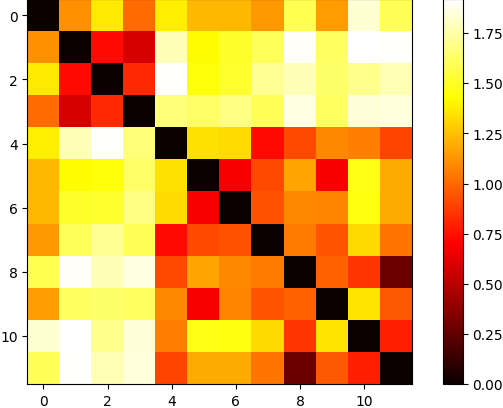
\includegraphics[width=\linewidth]{figures/syntetic_data/distance_matrix/SO3_signature_3.png}
        \caption{}
        \label{fig:classification-signature-level3-SO3}
    \end{subfigure}
    \hfill
    \begin{subfigure}{0.48\textwidth}
        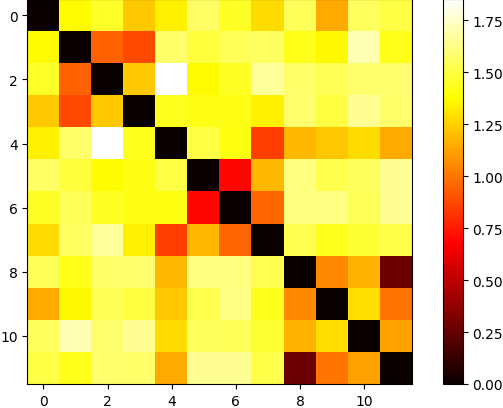
\includegraphics[width=\linewidth]{figures/syntetic_data/distance_matrix/SO3_signature_5.png}
        \caption{}
        \label{fig:classification-signature-level5-SO3}
    \end{subfigure}
    \vskip\baselineskip
    \begin{subfigure}{0.48\textwidth}
        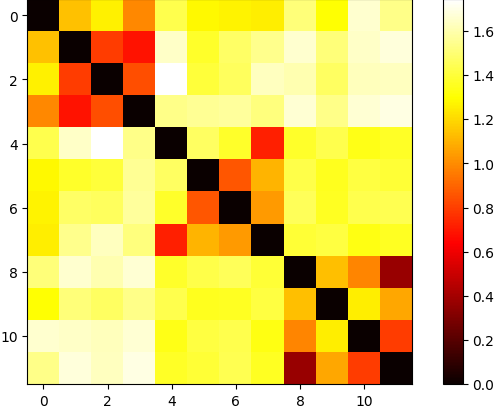
\includegraphics[width=\linewidth]{figures/syntetic_data/distance_matrix/SE3_signature_3.png}
        \caption{}
        \label{fig:classification-signature-level3-SE3}
    \end{subfigure}
    \hfill
    \begin{subfigure}{0.48\textwidth}
        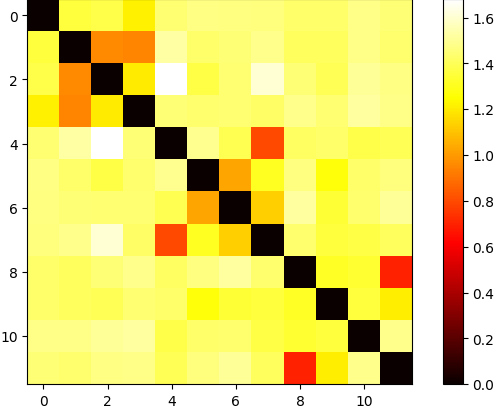
\includegraphics[width=\linewidth]{figures/syntetic_data/distance_matrix/SE3_signature_5.png}
        \caption{}
        \label{fig:classification-signature-level5-SE3}
    \end{subfigure}
    \caption[Classification using logarithmic signature on curves in \(\mathrm{SO}(3)\) and \(\mathrm{SE}(3)\)]{Distance matrices using the signature method for \(\mathrm{SO}(3)\) and \(\mathrm{SE}(3)\) at different truncation levels, visualized through the \(L^2\) norm between normalized signatures. Panels: (a) \(\mathrm{SO}(3)\), truncation level 3; (b) \(\mathrm{SO}(3)\), truncation level 5; (c) \(\mathrm{SE}(3)\), truncation level 3; (d) \(\mathrm{SE}(3)\), truncation level 5. These matrices illustrate the variation in signature-based classification accuracy across truncation levels.}
    \label{fig:classification-signature}
\end{figure}

\begin{figure}
    \centering
    \begin{subfigure}{0.48\textwidth}
        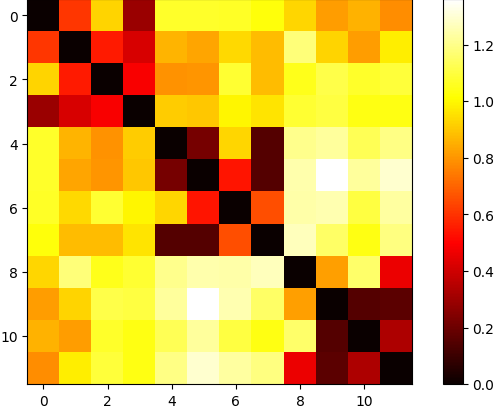
\includegraphics[width=\linewidth]{figures/syntetic_data/distance_matrix/SO3_3_signature_3.png}
        \caption{}
        \label{fig:classification-signature-level3-SO3-3}
    \end{subfigure}
    \hfill
    \begin{subfigure}{0.48\textwidth}
        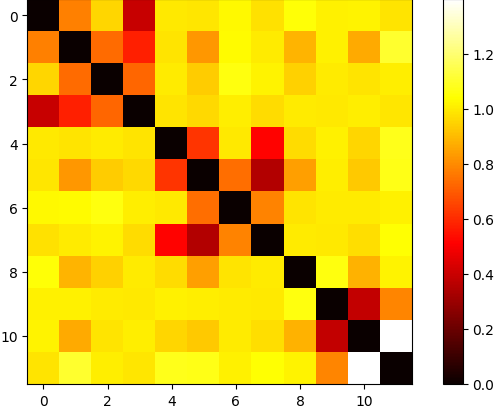
\includegraphics[width=\linewidth]{figures/syntetic_data/distance_matrix/SO3_3_signature_5.png}
        \caption{}
        \label{fig:classification-signature-level5-SO3-3}
    \end{subfigure}
    \vskip\baselineskip
    \begin{subfigure}{0.48\textwidth}
        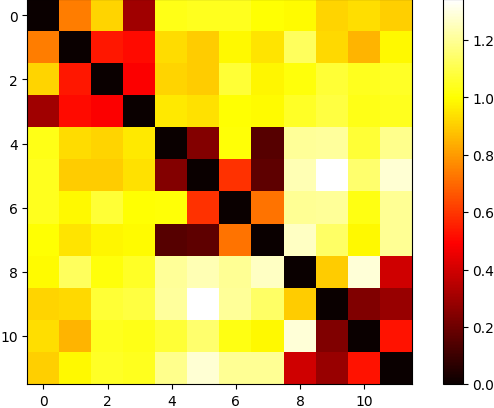
\includegraphics[width=\linewidth]{figures/syntetic_data/distance_matrix/SE3_3_signature_3.png}
        \caption{}
        \label{fig:classification-signature-level3-SE3-3}
    \end{subfigure}
    \hfill
    \begin{subfigure}{0.48\textwidth}
        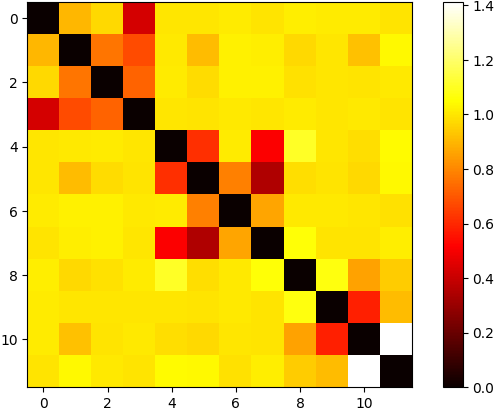
\includegraphics[width=\linewidth]{figures/syntetic_data/distance_matrix/SE3_3_signature_5.png}
        \caption{}
        \label{fig:classification-signature-level5-SE3-3}
    \end{subfigure}
    \caption[Classification using logarithmic signature on in \(\mathrm{SO}(3)^n\) and \(\mathrm{SE}(3)^n\)]{Distance matrices using the signature method for \(\mathrm{SO}(3)^3\) and \(\mathrm{SE}(3)^3\) at different truncation levels, visualized through the \(L^2\) norm between normalized signatures. Panels: (a) \(\mathrm{SO}(3)^3\), truncation level 3; (b) \(\mathrm{SO}(3)^3\), truncation level 5; (c) \(\mathrm{SE}(3)^3\), truncation level 3; (d) \(\mathrm{SE}(3)^3\), truncation level 5. These matrices illustrate the variation in signature-based classification accuracy across truncation levels.}
    \label{fig:classification-signature-3}
\end{figure}

In Figure \ref{fig:classification-signature}, it is evident that \(\mathrm{SE}(3)\) curves are more readily classified compared to \(\mathrm{SO}(3)\) curves, as shown by the more distinct clustering observed within the same geometric types. Increasing truncation levels in \(\mathrm{SO}(3)\) generally improves classification accuracy by incorporating more detailed information, resulting in a tighter grouping of curves with similar geometric characteristics. However, an interesting observation is made when the truncation level in \(\mathrm{SE}(3)\) is increased to 5: some curves from the same shape space unexpectedly exhibit large distances between them.

Figure \ref{fig:classification-signature-3} highlights the classification results for the spaces \(\mathrm{SO}(3)^n\) and \(\mathrm{SE}(3)^n\), which are notably promising. Distances within the same shape space remain low, indicating effective classification. Interestingly, classification performs better in \(\mathrm{SE}(3)^n\) than in \(\mathrm{SO}(3)^n\), demonstrating a superior ability to resolve geometric differences in these extended spaces. Similar to \(\mathrm{SE}(3)\), when the truncation level is increased to 5 in both \(\mathrm{SO}(3)^n\) and \(\mathrm{SE}(3)^n\), some curves from the same shape space begin to show significant distances between them.

These results highlight that the logarithmic signature is capable of distinguishing between curves of different shapes. By combining this with post-processing techniques, such as clustering, it may be possible to determine the shape of a curve based on its signature. However, the results also indicate that the choice of truncation level is crucial, as increasing the level may lead to unexpected results. Future work could explore the optimal truncation level for curve classification using the signature-based framework.

\subsection{Perturbation Analysis}
\label{subsec:perturbation-analysis-signature}

In this subsection, we investigate how the logarithmic signature-based distance metric (Equation \eqref{eq:signature-distance-metric}) behaves under perturbations. We utilize the curves \(c_i^\text{eq}\) and \(c_{i,i+1,i+2}^\text{eq}\) created in Subsection \ref{subsec:synthetic-data-generation}. To create a perturbed version of these curves, we solve the same differential equation \eqref{eq:diff-eq-synthetic}, but with timesteps perturbed by adding small, normally distributed noise. This results in the perturbed curves \(c_i^\epsilon\) and \(c_{i,i+1,i+2}^\epsilon\), with \(i \in \{1,2,3\}\) and \(i \in \{1,4,7\}\), respectively. We examine the effect of this perturbation on the signature-based distance metric by progressively reducing the standard deviation of the noise, performing this reduction 10 times. The results are shown in Figure \ref{fig:perturbation-analysis-signature}.

\begin{figure}
    \centering
    \begin{tikzpicture}
        \begin{loglogaxis}[
            width=0.8\textwidth,
            height=0.4\textwidth,
            xlabel={\(\epsilon\)},
            ylabel={\(d_{\mathcal{\text{sig}}_*}(c^\epsilon, c)\)},
            legend style={font=\small, at={(1.2,0.5)}, anchor=west},
            grid=major,
            legend pos=outer north east,
        ]
        
        \addplot [thick, red, solid] table [x=perturbation, y=c1, col sep=comma] {figures/syntetic_data/perturbation-analysis/signature-SO3.csv};
        \addlegendentry{\(\omega_0\)}

        \addplot [thick, blue, solid] table [x=perturbation, y=c2, col sep=comma] {figures/syntetic_data/perturbation-analysis/signature-SO3.csv};
        \addlegendentry{\(\omega_1\)}

        \addplot [thick, green, solid] table [x=perturbation, y=c3, col sep=comma] {figures/syntetic_data/perturbation-analysis/signature-SO3.csv};
        \addlegendentry{\(\omega_2\)}

        \addplot [thick, red, dashed] table [x=perturbation, y=c1, col sep=comma] {figures/syntetic_data/perturbation-analysis/signature-SE3.csv};
        \addlegendentry{\(\xi_0\)}

        \addplot [thick, blue, dashed] table [x=perturbation, y=c2, col sep=comma] {figures/syntetic_data/perturbation-analysis/signature-SE3.csv};
        \addlegendentry{\(\xi_1\)}

        \addplot [thick, green, dashed] table [x=perturbation, y=c3, col sep=comma] {figures/syntetic_data/perturbation-analysis/signature-SE3.csv};
        \addlegendentry{\(\xi_2\)}

        \logLogSlopeTriangle{0.7}{0.3}{0.2}{1}{black, dashed}
        
        \end{loglogaxis}
    \end{tikzpicture}
    \caption[Perturbation analysis plot of the logarithmic signature distance]{The signature based distance metric under perturbations in \(\mathrm{SO}(3)\) and \(\mathrm{SE}(3)\). The distance between the perturbed and non-perturbed curves is computed using the signature based distance metric. The curves are perturbed by adding a small normal distributed noise to the parameterization, where we halve the standard deviation, and the distance is computed 10 times.}
    \label{fig:perturbation-analysis-signature}
\end{figure}

We observe that as the perturbation size decreases, the signature-based distance metric also decreases. This indicates that the metric is robust to small perturbations, maintaining consistent performance even with minor noise in the parameterization of the curves.